The experiments consists of three sub experiments. In the first, baseline, experiment default evolutionary policy search is tested on the toy problem defined in section \ref{toyprob}. In the second experiment the effect of co-evolution is tested in order to validate the reduction of sample complexity and, thirdly, in the third experiment GP CEPS is applied. Lastly in order to analyze the certainty of the Gaussian Process, the predicted mean, upper bound and lower bound is examined when applying GP CEPS on the toy problem.

For all experiments the policy is a Neural Network with a hidden layer consisting of 4 hidden units, and the parameters are as defined in section \ref{evo_pol_search}. 

\subsection{Evolutionary Policy Search}

Figure \ref{Fitness during Evolutionary Algorithm} is the average result of ten runs. The x-axis shows the amount of epochs (evoluations), and the y-axis represents the return of the best performing policy in the pool where 95\% confidence intervals are shown. For each epoch five evaluations are done per organism, and the pool size is 20. For example the value 30 on the x-axis thus required $30 \times 5 \times 20 = 3000$ samples.

Figure \ref{Example policy learned with evolutionary algorithm} shows the behavior of an example policy found with the evolutionary policy search algorithm, after 200 epochs. The wind is sampled from a uniform distribution between 0 and 0.5. Note that for all wind strengths, this policy reaches the goal. 

\begin{figure}[!htb]
  \centering
  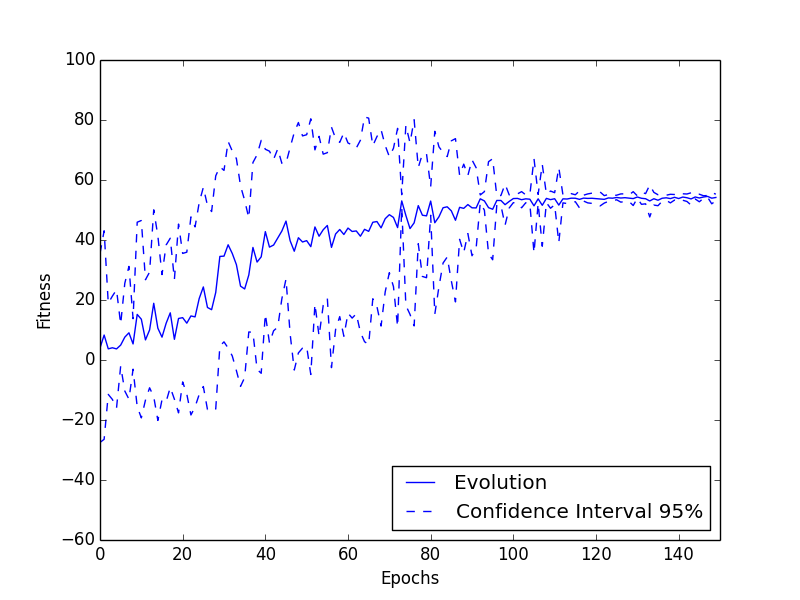
\includegraphics[scale=0.5]{images/evo.png}
  \caption{Fitness during Evolutionary Algorithm}\label{Fitness during Evolutionary Algorithm}
\end{figure}

\begin{figure}[!htb]
  \centering
  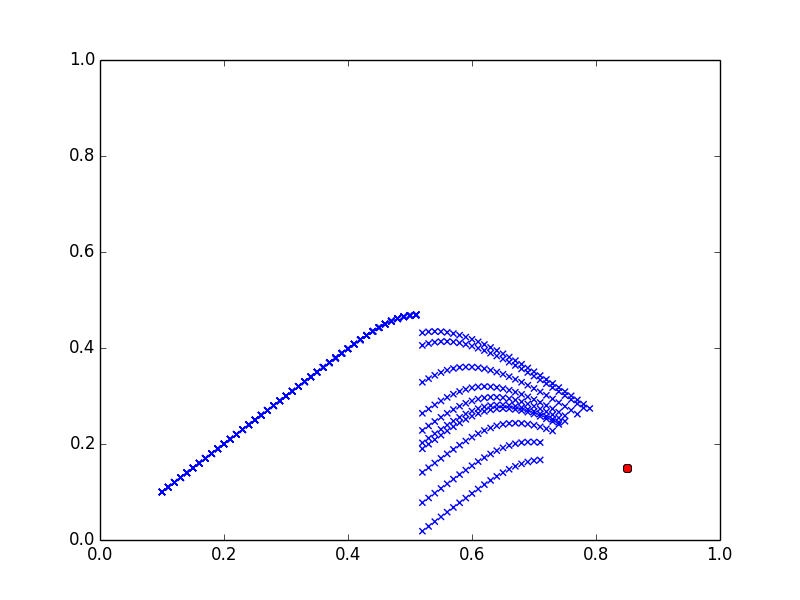
\includegraphics[scale=0.5]{images/evo_result.png}
  \caption{Example policy learned with evolutionary algorithm}\label{Example policy learned with evolutionary algorithm}
\end{figure}

\pagebreak
\subsection{Co-Evolutionary Policy Search}

The results for Co-Evolutionary Policy Search are shown in Figure \ref{Fitness during Co-Evolutionary Algorithm}. It converges to a similar reward as evolutionary policy search, although the learning curve is much steeper in the first epochs. In section \ref{comparisonSection} these two methods are compared more closely. For fair comparison the parameters are similar to the previous experiment: the wind is distributed uniformly between 0 and 0.5 and the same network structure is used. An example policy trained with Co-Evolutionary Policy Search for 200 epochs is visualized in Figure \ref{Example policy learned with Co-Evolutionary algorithm}. This policy, too, is able to reach the goal for any wind strength. The same sample complexity as in the first experiment applies.

\begin{figure}[!htb]
  \centering
  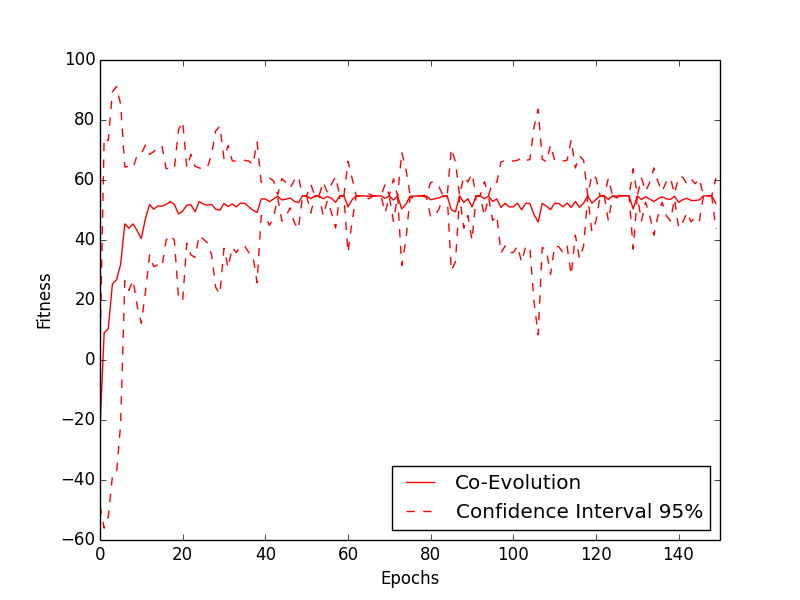
\includegraphics[scale=0.5]{images/co_evo.png}
  \caption{Fitness during Co-Evolutionary Algorithm}\label{Fitness during Co-Evolutionary Algorithm}
\end{figure}

\begin{figure}[!htb]
  \centering
  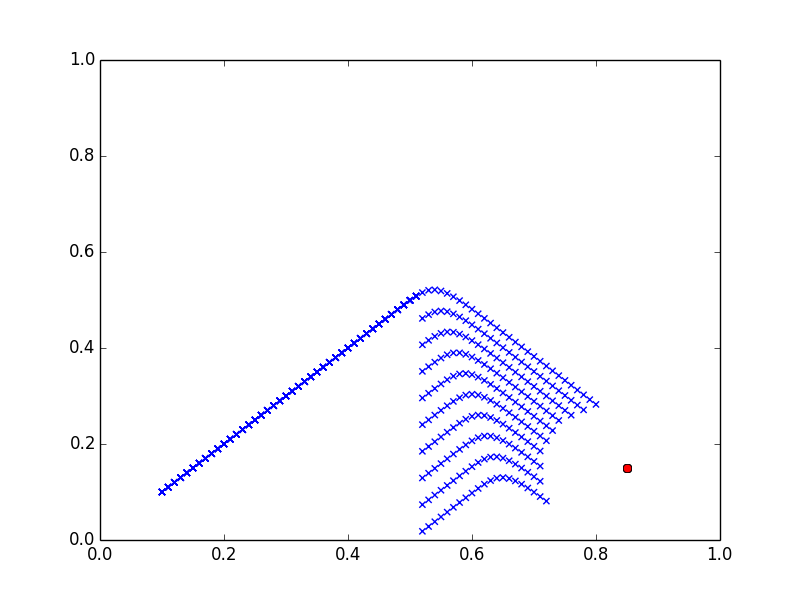
\includegraphics[scale=0.5]{images/co_evo_result.png}
  \caption{Example policy learned with Co-Evolutionary algorithm}\label{Example policy learned with Co-Evolutionary algorithm}
\end{figure}

\subsection{GP CEPS}

In this experiment we apply GP CEPS to the same problem. Figure \ref{Fitness during GP CEPS} shows the fitness of the policy found by using evolutionary policy search to find the policy with the highest predicted mean in the GP. The x-axis denotes the amount of samples. 

\begin{figure}[!htb]
  \centering
  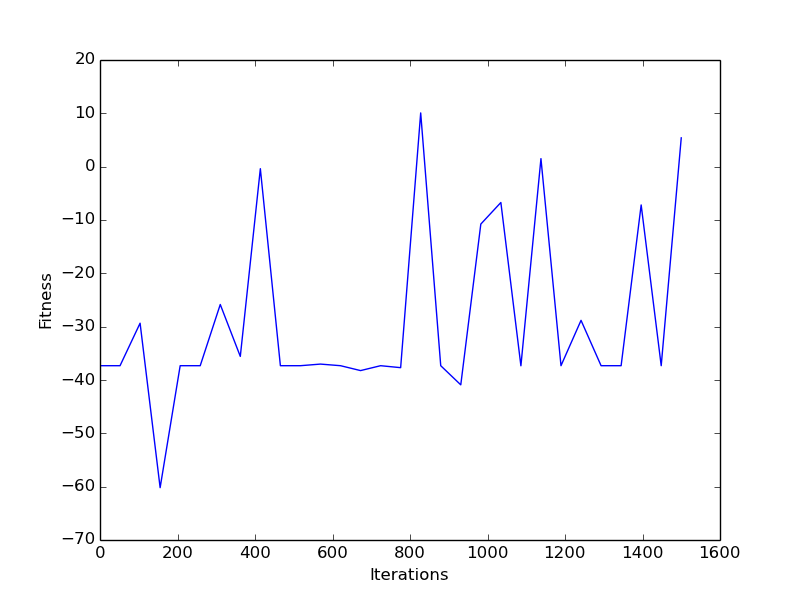
\includegraphics[scale=0.5]{images/GPCEPS_True.png}
  \caption{Fitness during GP CEPS}\label{Fitness during GP CEPS}
\end{figure}

An example of a policy generated by the GP CEPS approach is one in figure \ref{gp_policy}. It shows behavior similar to those found by the previous methods, but as it climbs less it is blown of from the grid more often it is a slightly worse policy. 

\begin{figure}[!htb]
  \centering
  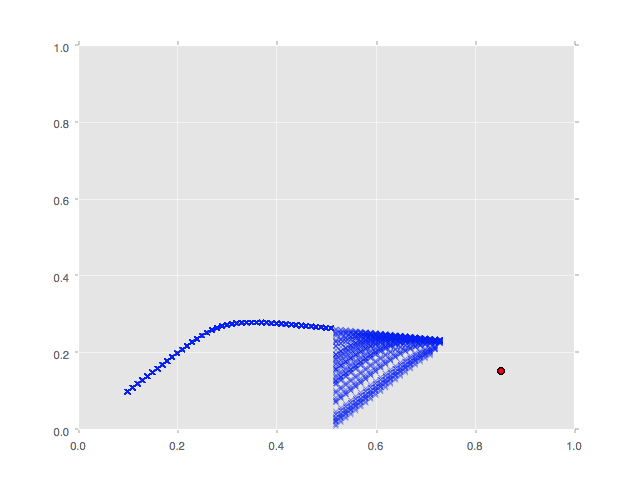
\includegraphics[scale=0.5]{images/GPCEPS_policy.png}
  \caption{Example policy learned with GP CEPS}\label{gp_policy}
\end{figure}

In addition the predicted mean, upper confidence bound (UCB) and lower confidence bound (LCB) is shown in figure \ref{pred_img}. We see that the GP is very uncertain about its predictions and that the mean does not increase over time.

\begin{figure}[!htb]
  \centering
  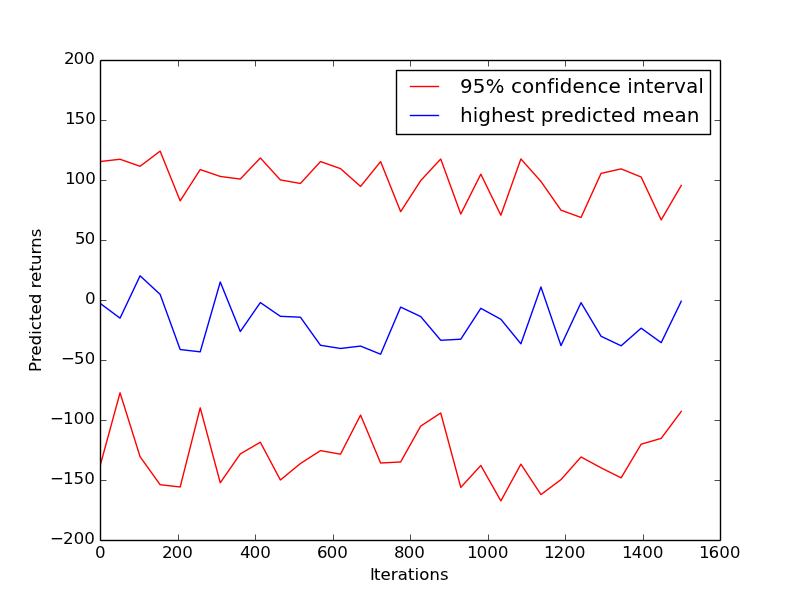
\includegraphics[scale=0.5]{images/GPCEPS_pred.png}
  \caption{Predicted mean, UCB and LCB during GP CEPS}\label{pred_img}
\end{figure}


\subsection{Comparison}\label{comparisonSection}
In order to better compare the two evolutionary methods (without a GP) their results are shown together in figure \ref{compare_img}. It shows co-evolution has a steeper learning curve, but both converge to the same value, which is the optimal value.

\begin{figure}[!htb]
  \centering
  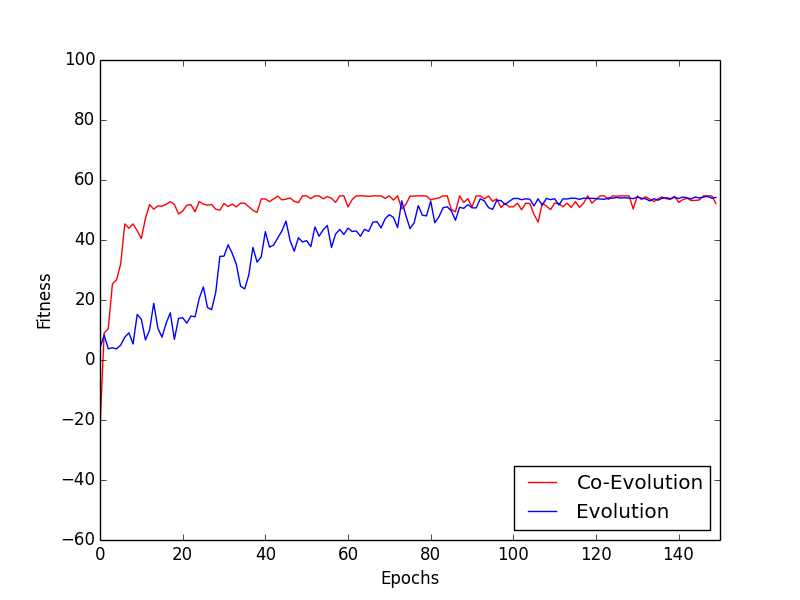
\includegraphics[scale=0.5]{images/together.png}
  \caption{Comparing the performance normal and co-Evulationary algorithms in required samples}\label{compare_img}
\end{figure}


